\section{Usage culinaire}

Toutes les grenouilles ne sont pas comestibles. 
Certaines espèces sont même toxiques et d'autres sont des espèces menacées de disparition dont les populations sont désormais protégées.

En cuisine française, ce sont les cuisses qui sont consommées. 
Les Français ont la réputation mondiale d'être des mangeurs de grenouilles, ce qui leur a valu leur surnom anglais de froggies, frog signifiant grenouille en anglais. 
Ainsi, on appelle $\ll$ Vallée des grenouilles $\gg$ un quartier de Londres, peuplé de beaucoup de Français.
En Italie les Français sont parfois appelés les mangiarane, c'est-à-dire les $\ll$ mangeurs de grenouilles $\gg$.

Traditionnellement, il s'agissait d'espèces locales, comme les grenouilles rousses (Rana temporaria) et vertes (Rana esculenta) désormais protégées à l'état sauvage en France, mais encore disponibles dans de rares élevages agréés. 
Elles ont été remplacées par des grenouilles asiatiques : Rana tigrina, Rana crassa et Rana catesbeiana quand elles sont surgelées et Rana ridibunda pour les importations vivantes.
D'autres pays d'Europe ou les États-Unis consomment également ces grenouilles d'importation.

Les autochtones au Cameroun mangent couramment Trichobatrachus robustus : chassé avec de longues lances, des machettes, et même parfois des armes à feu pour éviter ses griffes rétractiles, il finit alors au menu, rôti (entier). 
Dans les monts Rumpi, zone protégée à l'ouest du Cameroun, les autochtones en mangent les têtards, qui seraient assez gros.

\begin{figure}
	\begin{center}
		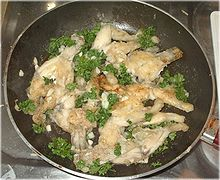
\includegraphics[scale=1]{cuisine/miam.JPG}
			\caption{Cuisses de grenouilles}
			\label{fig:gre}
	\end{center}
\end{figure}